\subsection{Architektura - wysokopoziomowo}\label{subsec:architektura-wysokopoziomowo}

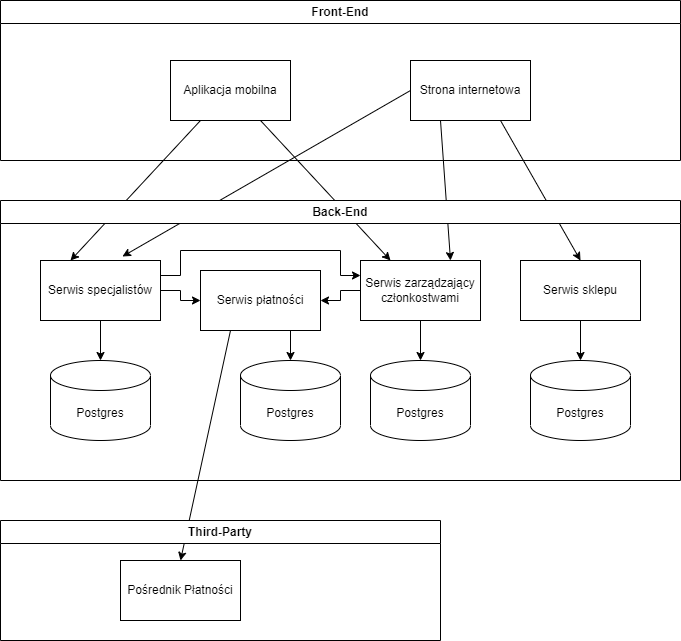
\includegraphics{../diagrams/architecture/high_level_architecture}

{System będzie składał się z aplikacji internetowej, która będzie służyła do zarządzania
siłownią. Strona będzie posiadała interfejs graficzny, który będzie
udostępniał funkcjonalności dla dwóch typów użytkowników: klientów oraz
pracowników siłowni. Klienci będą mogli przeglądać ofertę siłowni,
rezerwować zajęcia oraz kupować karnety. Pracownicy będą mogli dodawać
nowe zajęcia, edytować istniejące, dodawać nowe produkty do oferty
siłowni oraz zarządzać kontami klientów. Dodatkowo pracownicy będą posiadali możliwość
zarządzania sklepem jeśli tak jest dodany do siłowni.}

{Drugą częścią systemu od strony front-endu będzie aplikacja mobilna, która będzie służyła do wygodnego
przeglądania ofert specjalistów, zapisywania się na nie i kupowania karnetów. Specjaliści będą mogli
zarządzać własnymi wizytami.
Aplikacja będzie komunikowała się z dwoma serwisami back-endowymi - jednym do systemu specjalistów
oraz drugim do systemu karnetów.}

{Backend będzie składał się z wielu mikto-serwisów, które będą
komunikowały się ze sobą za pomocą protokołu HTTP. Każdy mikro-serwis
będzie posiadał własną bazę danych, która będzie przechowywała dane
specjalistów, zajęć, produktów oraz karnetów zależnie od potrzeb.}

{Warto wspomnieć, o serwisie płatności, który jako jedyny będzie potrzebował zewnętrzego API.
Musi on zintegrować się z pośrednikiem płatności, aby umożliwić klientom płatność za karnety.}

{Serwis sklepu nie zależy od reszty, gdyż pełni on jedynie rolę dokumentacji produktów i ich
ilości w magazynie.}
